\documentclass{beamer}

\usetheme{Luebeck}
\usepackage{CJKutf8}
\usepackage{graphicx}


\setcounter {tocdepth}{ 3}
\title{Final Presentation}

\begin{document}

\begin{frame}
  \titlepage
\end{frame}



   \tableofcontents






\section{Producing presentation slides using the LaTex \medskip}
\begin{frame}{Producing presentation slides using the LaTex}
	(Fig.\,\ref{fig:1} )
    \begin{figure}
    \caption{1}
    \label{fig:1}
  \end{figure}
\end{frame}


\section{Content includes the following }

\subsection{Introduction}

\subsubsection{Introduction to your team}
\begin{frame}{Introduction to your team}
\begin{itemize}
  \item  \begin{CJK}{UTF8}{bkai}1053311 李厚徵\end{CJK}
  \item  \begin{CJK}{UTF8}{bkai}1041517 桑翊軒\end{CJK}
  \item \begin{CJK}{UTF8}{bkai}1053312 陳冠廷\end{CJK}
  \item  \begin{CJK}{UTF8}{bkai}1051535 楊宗霖\end{CJK}
  \item  \begin{CJK}{UTF8}{bkai}1053318 張嘉祐\end{CJK}
\end{itemize}
\end{frame}

\subsubsection{Introduction to the problem you're trying to solve \medskip}
\begin{frame}{Introduction to the problem you're trying to solve}
  \begin{CJK}{UTF8}{bkai}
  \linespread{1.5}\selectfont
	\qquad 期末專題主要是想解決我們對大自然的好奇心,
	當我們在校園探索當中,有很多花我們不知道其名稱,
	透過這門課所學的知識,利用影像辨識的方法,將各種花朵辨識出來。
  \end{CJK}
\end{frame}

\subsection{Methodology}
\subsubsection{ Input of your model }
\begin{frame}{Input of your model }
  (Fig.\,\ref{fig:2} )
    \begin{figure}
    \caption{2}
    \label{fig:2}
  \end{figure}
\end{frame}

\subsubsection{Output of your model }
\begin{frame}{Output of your model }
  \begin{CJK}{UTF8}{bkai}
	Prediction result(包含: 預測的label, 其信心度)(Fig.\,\ref{fig:3} )
    \begin{figure}
      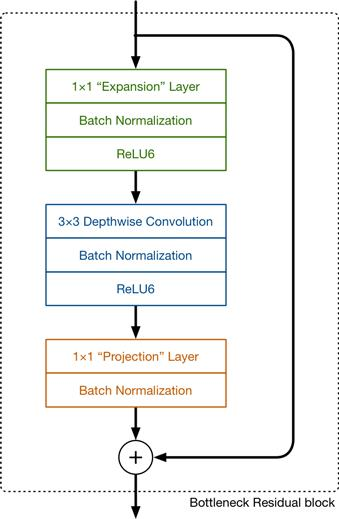
\includegraphics[width=0.3\linewidth]{layer.jpg}
      \caption{3}
      \label{fig:3}
    \end{figure}
   \end{CJK}
\end{frame}

\subsubsection{Each layer of your model }
\begin{frame}{Each layer of your model }
	Expansion layer, convolution layer, projection layer… (Fig.\,\ref{fig:4} )
  \begin{figure}
    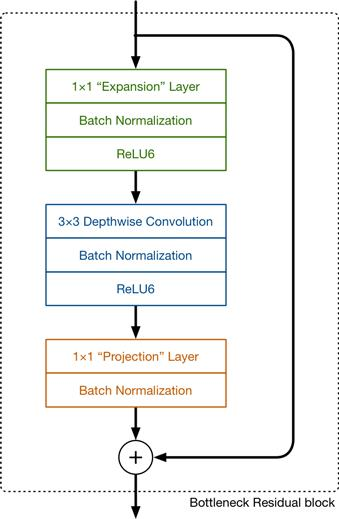
\includegraphics[width=0.3\linewidth]{layer.jpg}
    \caption{4}
    \label{fig:4}
  \end{figure}
\end{frame}

\subsubsection{How you save your model? }
\begin{frame}{How you save your model? }
  \begin{CJK}{UTF8}{bkai}
	We save as filename.pb(pb檔)
   \end{CJK}
\end{frame}

\subsubsection{File size of your mode }
\begin{frame}{File size of your model }

\end{frame}

\subsubsection{What's your loss functions, and why?}
\begin{frame}{What's your loss functions, and why?}

\end{frame}

\subsubsection{What's your optimizer and the setting of hyperparameter?  \bigskip \bigskip \bigskip \bigskip}
\begin{frame}{What's your optimizer and the setting of hyperparameter? }

\end{frame}
%stop


\subsection{Dataset}
\subsubsection{The size of your dataset should be larger than 1K}
\begin{frame}{The size of your dataset should be larger than 1K}

\end{frame}
\subsubsection{How you collect/build your dataset?}
\begin{frame}{How you collect/build your dataset?}
  \begin{CJK}{UTF8}{bkai}
	對花做360度的影片拍攝,再將影片以frame切割。
   \end{CJK}
\end{frame}

\subsubsection{How many paired training samples in your dataset?}
\begin{frame}{How many paired training samples in your dataset?}

\end{frame}

\subsubsection{How many paired validating samples in your dataset?}
\begin{frame}{How many paired validating samples in your dataset?}

\end{frame}

\subsubsection{How many paired testing samples in your dataset?}
\begin{frame}{How many paired testing samples in your dataset?}

\end{frame}

\subsection{Experimental Evaluation }
\subsubsection{Experimental environment (CPU, GPU, memory,…,etc.)}
\begin{frame}{Experimental environment (CPU, GPU, memory,…,etc.)}
CPU
\end{frame}

\subsubsection{How many epochs you set for training?}
\begin{frame}{How many epochs you set for training?}
4000
\end{frame}

\subsubsection{Qualitative evaluation}
\begin{frame}{Qualitative evaluation}

\end{frame}

\subsubsection{Quantitative evaluation}
\begin{frame}{Quantitative evaluation}

\end{frame}

\subsection{Live demo of your work}
\begin{frame}{Live demo of your work}

\end{frame}















\end{document}